\section{Deployment and orchestration}\label{sec:deployment-and-orchestration}
In order to overcome the issues described in the section \ref{sec:performance-tests}, the cloud providers' research was conducted, and based on the results it was decided to adopt the \gls{gcp} (Google Cloud Platform)\upperref{itm:gcp} as a deployment environment.

Unlike Heroku, \gls{gcp} had no free pricing plan, but it does not restrict the usage of resources and therefore it met the project assumptions, and moreover, it has some extra advantages like native support for containers orchestration.
The latter is provided by using Kubernetes\upperref{itm:kubernetes}, the open-source solution introducing flexible deployments, scaling and container management.
Those features drastically simplify working with application development in a cloud but require additional setup and configuration files.

Kubernetes natively supports the usage of Docker containers so the ones prepared before can be reused, but the deployment process requires a so-called Deployment configuration files that enable tuning the resources assigned to the single instance of an application and also the number of the replicas of the application.
The basic unit managed by Kubernetes is Pod which may consist of many single Docker containers, but in this work the Pod is associated with a single container of application.
The described scaling method is known as Horizontal Pod Scaling and can be seen in the Fig.~\ref{fig:gcp_diagram} as a several same Pods in single Deployment.
It improves reliability and allows to increase the limit of the maximal load accepted by a single deployment of the application because the load is split into the mirror instances of the same application that work in parallel.
In Fig.~\ref{fig:gcp_diagram} the Deployments are draw as rectangles which states that all of their content is in some measure related to them.

\begin{figure}
    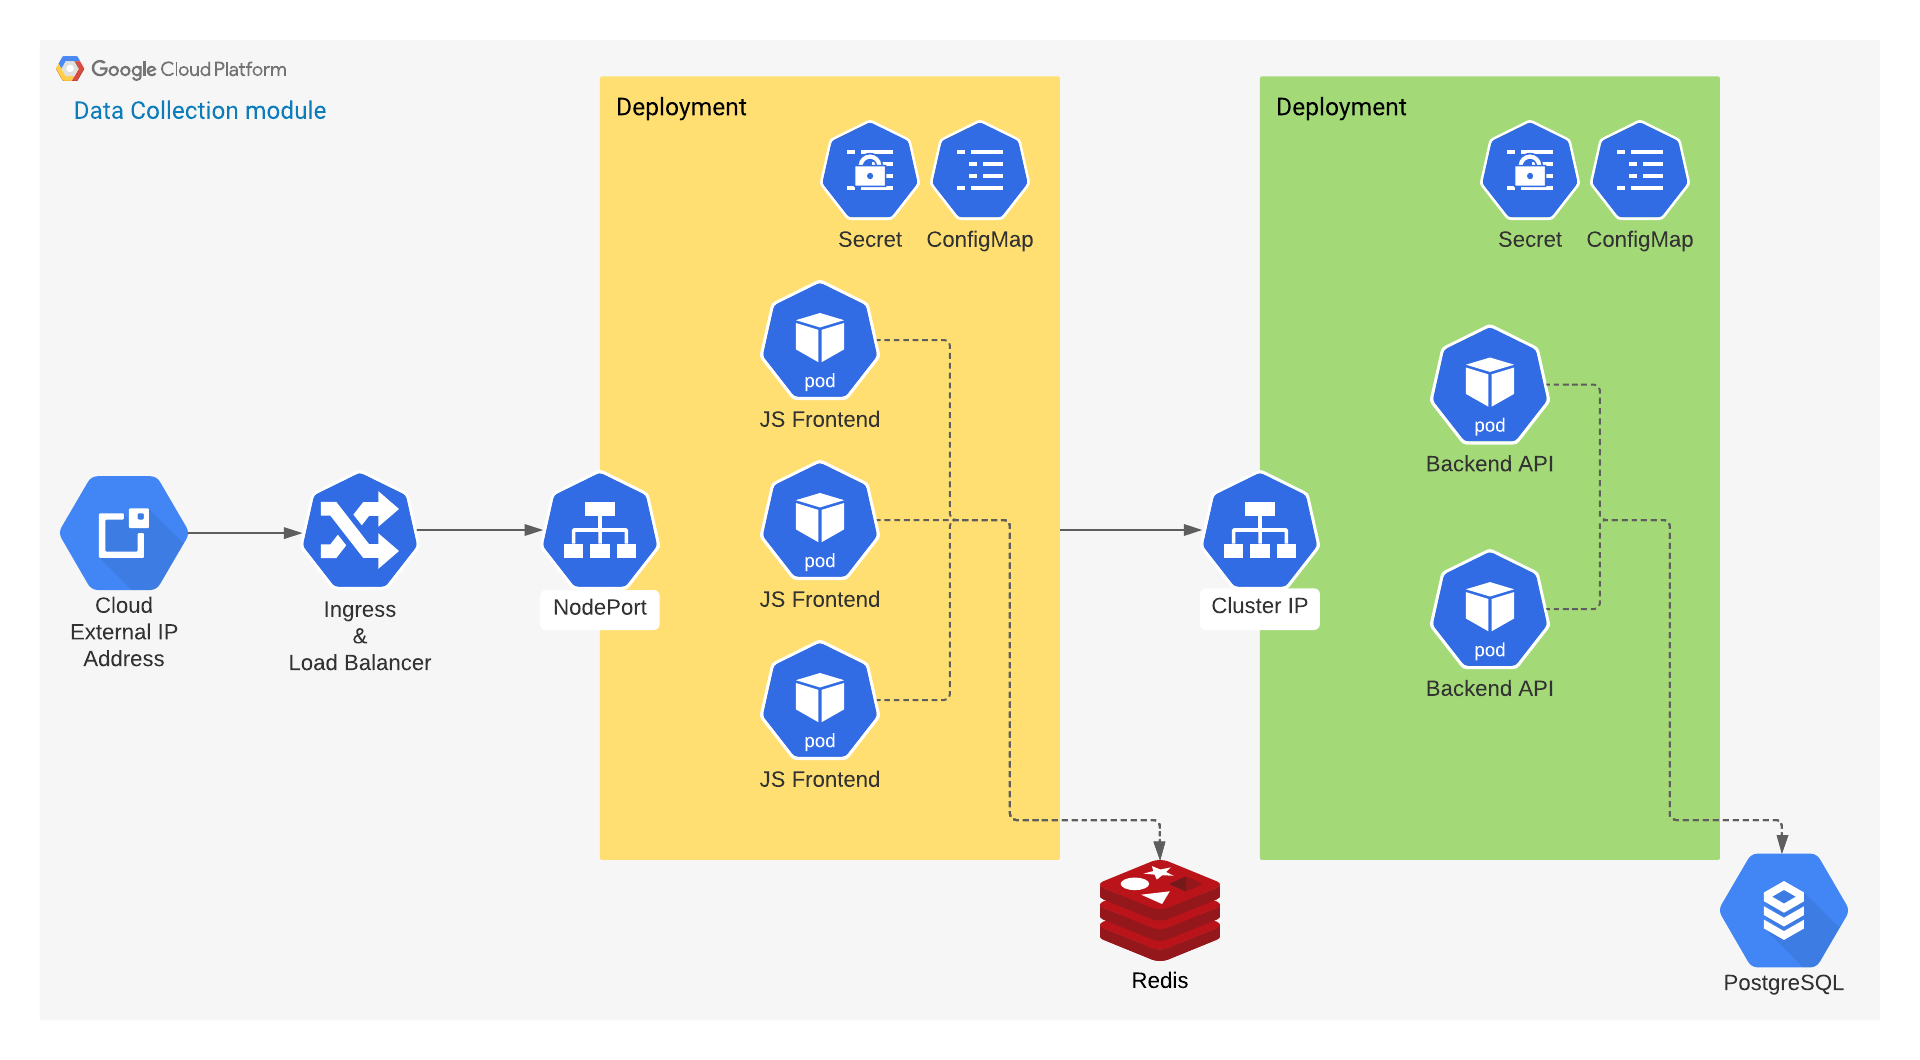
\includegraphics[width=\linewidth]{resources/gcp_diagram}
    \captionof{figure}{Cloud architecture}
    \label{fig:gcp_diagram}
\end{figure}

To deliver the load to all of the mirror applications, Kubernetes uses Services as an entry point to a group of Pods that are managed by one Deployment (in the Fig.~\ref{fig:gcp_diagram} they are drawn on the edge of the Deployment rectangles to mark their gateway nature).
The Service exposes the Deployment under the single \gls{dns} name and updates the underlying IP address in cases of its change, but it also works as a load balancer which distributes the load among the managed Pods.
Kubernetes has several different Service types but in this work two of them are used: Cluster IP that exposes the Deployments in the scope of Kubernetes but hides them from external access and NodePort that permits the access using port-forwarding.
The latter one is dictated by the usage of Google Cloud HTTP(S) load balancer and it also requires additional configuration by using an Ingress and obtaining the static external IP address.

To provide encryption of connection, \gls{tls} should be used, which requires the \gls{ssl} Server Certificate, which can be issued only for existing valid domain names, thus the authors were forced to buy such a domain name, while the certificate is issued by \gls{gcp}.

The configuration also includes some sensitive data, such as database credentials, OAuth2 secret, and SSH-RSA keys, thus the Secrets are used with encoded content.
The insensitive data are included in ConfigMaps that are similar to the Secrets but their content is plain text.
These configurations are matched to the appropriate component by labels and therefore they are drawn inside the Deployment rectangles in Fig.~\ref{fig:gcp_diagram}, in practice they can be mounted as volumes basing on the component labels and can also expose their values as environmental variables.

The whole architecture of the collector system is presented in Fig.~\ref{fig:gcp_diagram}, but the figure has several simplifications such as a way of database deployment.
In contrast to the Redis cache database, the main database instance is not deployed in Kubernetes itself, but the Cloud SQL from \gls{gcp} available services with \mbox{PostgreSQL} is used to achieve straightforward management and reliability.
